\subsection{Introduction}
A polynomial in the variable x over an algebraic field $F$ represents a function 
$A(x)$ as a formal sum:
\[A(x) = \sum_{j = 0}^{n-1} a_j x^j\]
We call the values $a_0, ~a_1, ~\cdots, ~a_{n-1}$ the \textbf{coefficients} of 
the polynomial. The coefficients are drawn from a field $F$ , typically the set 
$\mathbb{C}$ of complex numbers. A polynomial can be represented as a list of 
coefficients in computer.

A polynomial $A(x)$ has \textbf{degree $k$} if its highest nonzero coefficient 
is $a_k$. We write that $\text{degree}(A) = k$. Any integer strictly greater 
than the degree of a polynomial is a \textbf{degree-bound }of that polynomial. 
Therefore, the degree of a polynomial of degree-bound $n$ may be any integer 
between $0$ and $n-1$, inclusive.

Polynomial Multiplication: if $A(x)$ and $B(x)$ are polynomials of degree-bound 
$n$, their product $C(x)$ is a polynomial of degree-bound $2n - 1$ such that
$C(x) = A(x)B(x)$ for all $x$ in the underlying field. For example,

\centerline{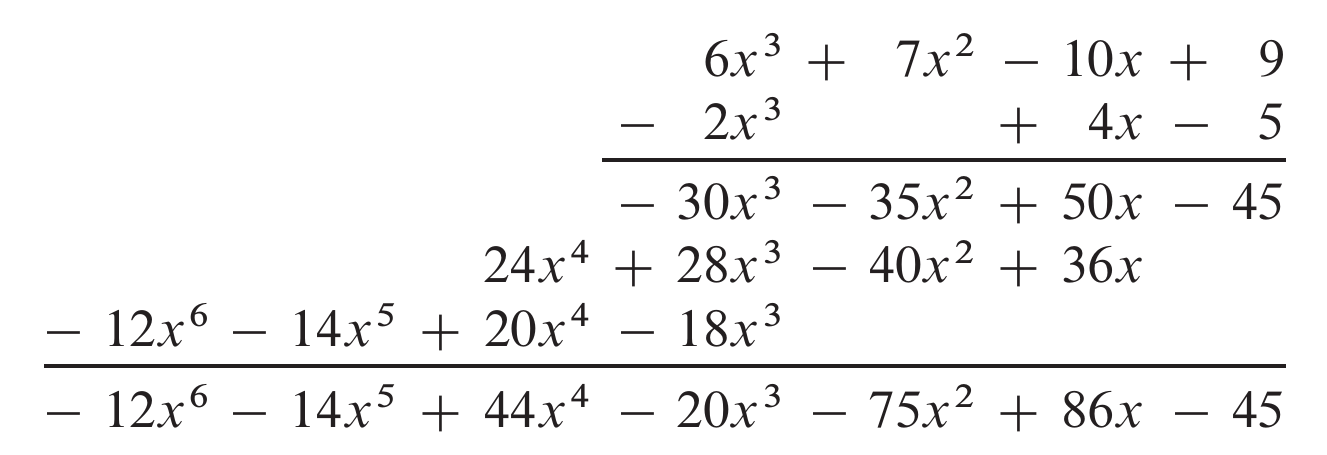
\includegraphics[width=0.5\textwidth]{poly-multiply.png}}

Another way to express the product $C(x)$ is
\begin{align*}
 C(x) = \sum_{j=0}^{2n-2} c_j x^j\\
 \intertext{where}
 c_j = \sum_{k=0}^j a_k b^{j-k}
\end{align*}

Note that $\text{degree}(C) = \text{degree}(A) +  \text{degree}(B)$, implying 
that if $A$ is a polynomial of degree-bound $n_a$ and $B$ is a polynomial 
of degree-bound $n_b$ , then $C$ is a polynomial of degree-bound $n_a + n_b - 
1$. Since a polynomial of degree-bound $k$ is also a polynomial of degree-bound 
$k + 1$, we will normally say that the product polynomial $C$ is a polynomial 
of degree-bound $n_a + n_b$.

\subsection{Algorithm}
Input: Two polynomials with same degree $d$:
\begin{align*}
 A &= a_d x^d + \cdots + a_0\\
 B &= b_d x^d + \cdots + b_0
\end{align*}
Goal: Calculate the product of the inputs.

\subsubsection{Baseline Method}
Simply calculate each parameter based on the definition of polynomial product. 
Each parameter in $A(x)$ should multiply all the parameters in $B(x)$ 
which takes $O(n^2)$ steps.
\subsubsection{Divide and Conquer}
\textbf{Assumption}: To make sure the parameters could be nicely divided by 
two, we assume the degree $d$ of both polynomials is always $2^k - 1$, where $k 
\in \mathbb{N}$.

Divide the $(d+1)$ entries of polynomials as follows to reduce the problem size:

\centerline{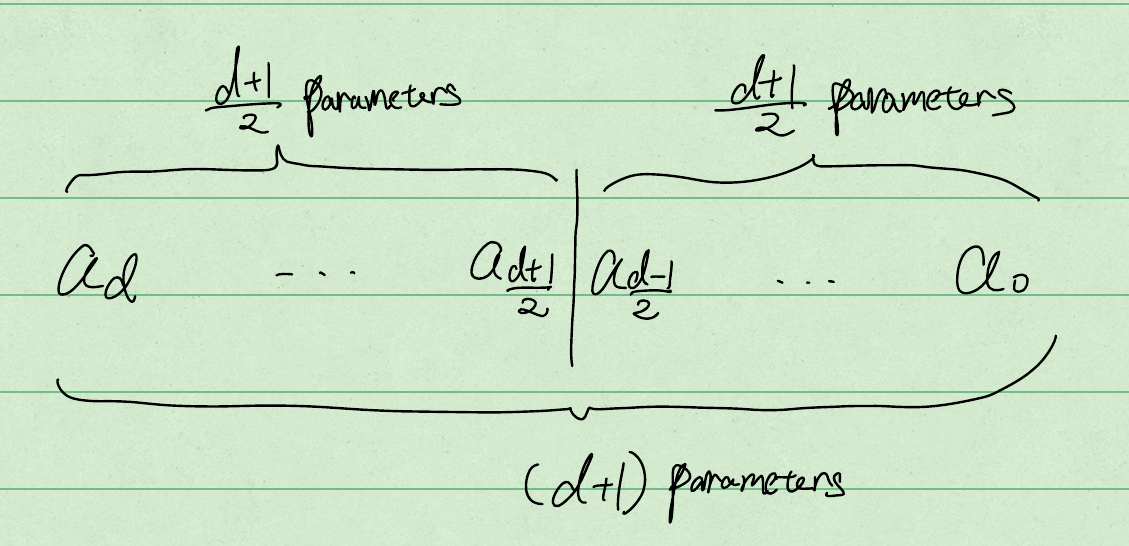
\includegraphics[width=0.5\textwidth]{poly-devide.png}}

Call the right hand side of polynomial as $A_l$. Extract $x^{\frac{d+1}{2}}$ 
and call the left hand side of polynomial as $x^{\frac{d+1}{2}} A_h$. we have,
\begin{align*}
 A &= x^{\frac{d+1}{2}} A_h + A_l\\
 B &= x^{\frac{d+1}{2}} B_h + B_l\\
 \intertext{Based on the algebra,}
 A \times B &= (x^{\frac{d+1}{2}} A_h + A_l)(x^{\frac{d+1}{2}} B_h + B_l)\\
 &= x^{d+1}A_h B_h + x^{\frac{d+1}{2}}A_h B_l + x^{\frac{d+1}{2}}A_l B_h + A_l 
B_l
\end{align*}
Therefore, we reduce the problem into four sub-problems with half of the size. 
Suppose the number of parameters is $n$, i.e. the degree of polynomials is $d = 
n - 1$. The recursion equation as follows:
\[T(n) \le 4T(\frac{n}{2}) + cn\]
Based on master theorem, $T(n) = O(n^2)$. Unfortunately, we have not get any 
improvement from those nicely splits comparing with the baseline. If you think 
about it, the result is actually not surprising because even though the problem 
size is reduced, we could not skip any of the necessary multiplication. In 
other words, there are still $n^2$ necessary multiplications to get the 
production.

\textbf{Motivation}: When you have a recursive algorithm, saving  one operation 
could have a cascade effect and reduce the run time quickly. Adding polynomials 
only costs $O(n)$ steps. If we could reduce multiplications by introducing 
addition. Then we are able to achieve better performance. 

To reduce the multiplications by adding additions, we have
\begin{align*}
 A \times B &= x^{d+1}A_h B_h + x^{\frac{d+1}{2}}A_h B_l + x^{\frac{d+1}{2}}A_l 
B_h + A_lB_l\\
            &= x^{d+1}A_h B_h + x^{\frac{d+1}{2}}(A_h B_l + A_l B_h) + A_l 
B_l
\end{align*}
Therefore, there are three items to calculate
\begin{enumerate}[(1)]
 \item $A_h B_h$
 \item $A_l B_l$
 \item $A_h B_l + A_l B_h$
\end{enumerate}
(1) and (2) are two multiplications. Moreover, (3) can be calculate by one more 
multiplication as following:
\begin{align*}
 &  (A_h + A_l) (B_h + B_l) - A_h B_h - A_l B_l\\
 =& A_hB_h + A_hB_l + A_lB_h + A_lB_l - A_h B_h - A_l B_l\\
 =& A_lB_h + A_hB_l
\end{align*}

Therefore, the recursive function becomes
\[T(n) \le 3T(\frac{n}{2}) + cn\]
It can be solved by master theorem, where $a = 3, b = 2, c = 1$.

Since $\log_ba > 1 = c$, so $T(n) = O(n^{\log_2 3}) \approx O(n^{1.6})$